\lhead{\textbf{Basic Algorithms, Fall 2024 \\ CSCI-UA.0310-001}}
\chead{\Large{\textbf{Homework 8}}}
\def\lc{\left\lceil}   
\def\rc{\right\rceil}
%%%%%%%%%%%%%%%%%%%%%%%%%%%%%%%%%%%%%%%
% ENTER NAME BELOW!
%%%%%%%%%%%%%%%%%%%%%%%%%%%%%%%%%%%%%%%
\rhead{\textbf{Instructor: Rotem Oshman \\Name: Ishan Pranav}}
\runningheadrule
\firstpageheadrule
\cfoot{}
\stepcounter{subsection}

\vspace*{-1em}
Peer-reviewed with Crystal Huang.

\subsection{Breadth-first search}
Recall the {\sc BFS} algorithm from the lecture that runs on graph $G$ starting from root node $s \in V$:
\begin{code}
    {\sc BFS}$(G,s)$\\
    1 \> $s.color = gray$, $s.dist = 0$. \\
    2 \> \For $u \in V \setminus \{s\}$ \\
    3 \> \> $u.color = white$, $u.dist = \infty$ \\
    4 \> $Q = \emptyset$ \\
    5 \> $Q.enqueue(s)$ \\
    6 \> \While $Q \neq \emptyset$ \\
    7 \> \> $u = Q.dequeue()$ \\
    8 \> \> \For $v \in Adj[u]$ \\
    9 \> \> \> \If $v.color = white$ \\
    10 \> \> \> \> $v.color = gray$ \\
    11 \> \> \> \> $v.dist = u.dist+1$ \\
    12 \> \> \> \> $Q.enqueue(v)$ \\
    13 \> \> $u.color = black$
\end{code}


\begin{enumerate}
    \item Consider the undirected graph shown in Figure~\ref{fig:box}.
    If we begin a BFS traversal starting at node $A$, in what order are the nodes visited? Assume that the adjacency list is ordered alphabetically, i.e., we visit earlier letters alphabetically first, so from $A$ we will visit $B$ before $C$, and so on.
    
    \begin{figure}[h]
        \centering
        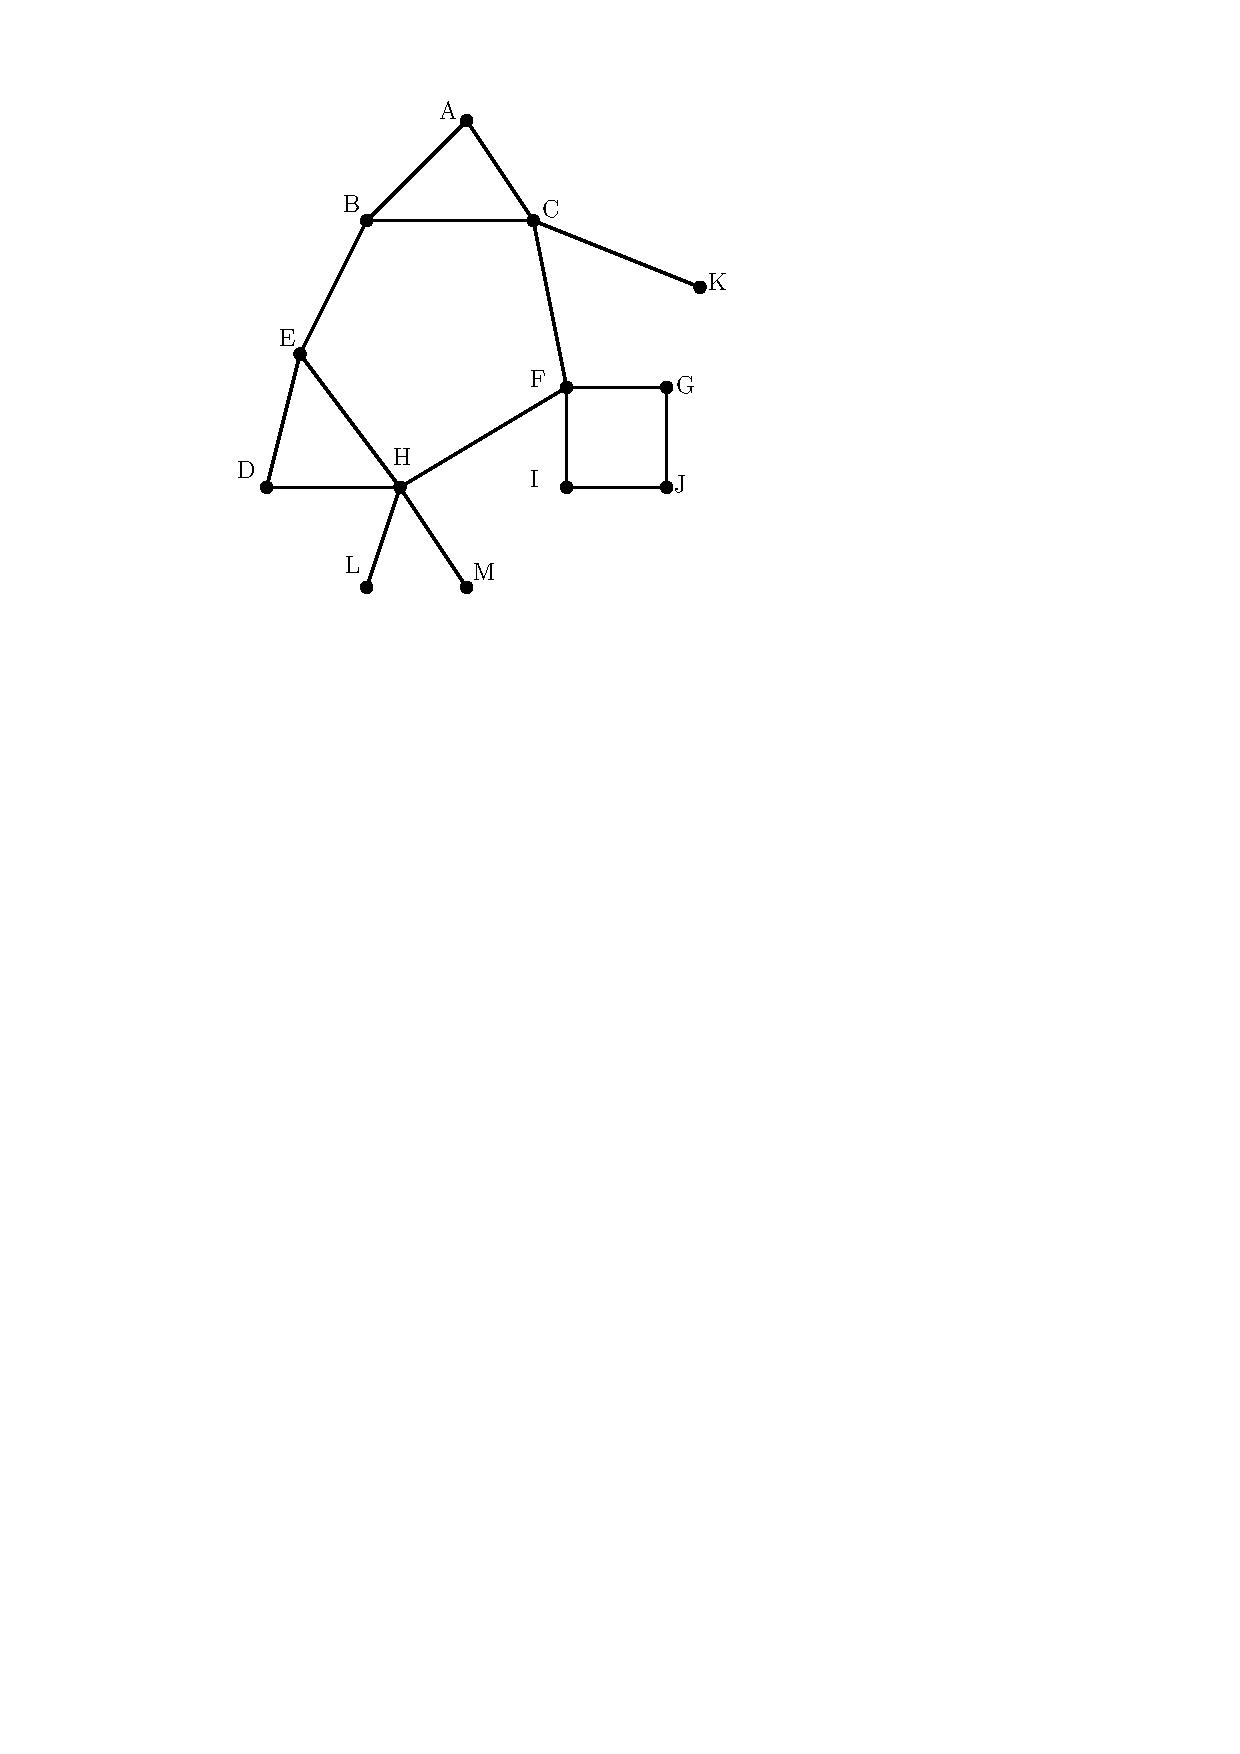
\includegraphics[width=0.4\textwidth]{images/BFS.pdf}
        \caption{Graph to traverse}
        \label{fig:box}
    \end{figure}
    
\begin{solution}

\end{solution}
\item Explain what happens if we don't check whether a node is white before enqueuing it.
\begin{solution}   INSERT YOUR SOLUTION HERE   \end{solution}

    \item Assume we replace the (FIFO) queue with a stack and therefore in line 7 obtain the node \emph{last} added. Does $v.dist$ still represent the shortest distance from $s$ to $v$?
\begin{solution}   INSERT YOUR SOLUTION HERE   \end{solution}

    \item Consider graphs for which edges have assigned weights. Assume we modify line 11 of BFS to add the weight of the edge from $u$ to $v$ instead of adding $1$. Does the modified algorithm compute the shortest weighted distance correctly? If so, prove the correctness; otherwise, provide a counterexample for which the algorithm fails.
\begin{solution}   INSERT YOUR SOLUTION HERE   \end{solution}
    
\end{enumerate}
\newpage
\subsection{Universal sink}
Recall that the \emph{adjacency matrix} representation of a \emph{directed} graph $G=(V,E)$ is the $|V| \times |V|$ matrix $M_G$ where $M_G[i][j]$ is $1$ if there is an edge from vertex $i$ to vertex $j$, and $0$ otherwise.
You may assume no vertex in the graph has an edge going into itself (i.e., no self-loops). We want to determine whether there is any vertex in $G$ that has edges coming to it from \emph{all other} vertices but no edges going out from it (this is known as a \textbf{universal sink}). 

\begin{enumerate}
\item Write an $O(|V|^2)$ algorithm that, given $M_G$, checks if there is a universal sink.
\begin{solution}

\textbf{Algorithm I. }{\sc IsSink}($M_G,v$) with a $|V|\times|V|$ adjacency matrix $M_G$ representing directed graph $G=(V,E)$ and a vertex $v\in V$; returns \verb|true| if $v$ is a universal sink; otherwise, \verb|false|:

For $u\in V$:
\begin{itemize}
    \item if $u=v$, then continue to next $u$;
    \item if $M_G[v,u]=1$ and $M_G[u,v]=0$, then return \verb|false|.
\end{itemize}
Return \verb|true|.

\textbf{Algorithm II. }{\sc QuadraticSink}($M_G$) with a $|V|\times|V|$ adjacency matrix $M_G$ representing directed graph $G=(V,E)$; returns \verb|true| if there is a universal sink in $G$; otherwise, \verb|false|:

For $v\in V$:
\begin{itemize}
\item If {\sc IsSink}($M_G,v$) is \verb|true|, then return \verb|true|.
\end{itemize}
Return \verb|false|.

\textbf{Proposition I. }\textit{Claim. }Algorithm I determines if $v$ is a universal sink in $G$ in running time $O(|V|)$.

\textit{Proof. }By definition, $v$ is a universal sink in $G=(V,E)$ if, for all $u\in V$ where $u\neq v$, we have $(u,v)\in E$ but $(v,u)\notin E$. The {\sc IsSink} algorithm compares $v$ to all other vertices $u$ and returns \verb|true| only if $v$ has edges coming to it from all other vertices $u$ and no edge going out from it to any vertex $u$. Otherwise, {\sc IsSink} returns \verb|false|. Thus, Algorithm I correctly determines if $v$ is a universal sink.

This implementation of Algorithm I visits every element in $V$ and performs constant-time operations within the loop body, so it has running time $O(|V|\times 1)=O(|V|).~\square$

\textbf{Proposition II. }\textit{Claim. }Algorithm II determines if there exists a universal sink in $G$ in running time $O(|V|^2)$.

\textit{Proof. }For $G=(V,E)$, The {\sc QuadraticSink} algorithm checks every vertex $v\in V$, using Algorithm I to determine if $v$ is a universal sink. From Proposition I, Algorithm I correctly determines if $v$ is a universal sink. Since Algorithm II returns \verb|true| if Algorithm I determines that any vertex is a universal sink (and \verb|false| if none satisfies this test), Algorithm II correctly determines if there exists a universal sink in $G$.

This implementation of Algorithm II visits every element in $V$ and performs {\sc IsSink} on each ($O(|V|)$ by Proposition I) within the loop body, so it has running time $O(|V|\times |V|)=O(|V|^2).~\square$
\end{solution}
\item Write an $O(|V|)$ algorithm for the problem. Justify why it is correct, as well as why it satisfies this run-time bound. 
\hint{Notice that for any pair of vertices $i,j$, the edge $i\rightarrow j$ is either present or absent. If it is present, then $i$ cannot be a universal sink. If it is absent, then $j$ cannot be a universal sink. Justify this fact and use it to create your algorithm.}
\begin{solution}
\textbf{Algorithm III. }{\sc LinearSink}($M_G$) with a $|V|\times |V|$ adjacency matrix $M_G$ representing directed graph $G=(V,E)$; returns \verb|true| if there is a universal sink in $G$; otherwise, \verb|false|:

Let $v^*\leftarrow v\in V$, choosing $v$ arbitrarily.

Let $U\leftarrow V\setminus\{v^*\}$.

For $u\in U$:
\begin{itemize}
\item if $M_G[v^*][u]=1$, then assign $v^*\leftarrow u$.
\end{itemize}

Return {\sc IsSink}($M_G,v^*$).

\textbf{Invariant I. }\textit{Claim. }

\textit{Proof. }

\textbf{Proposition III. }\textit{Claim. }Algorithm III determines if there exists a universal sink in $G$ in running time $O(|V|)$.

\textit{Proof. }
\end{solution}
\end{enumerate}
